\documentclass[12pt]{article}
\usepackage{amsmath}
\usepackage{latexsym}
\usepackage{amsfonts}
\usepackage{amssymb}
\usepackage{graphicx}
\usepackage{txfonts}
\usepackage{wasysym}
\usepackage{adjustbox}
\usepackage{ragged2e}
\usepackage{tabularx}
\usepackage{hhline}
\usepackage{float}
\usepackage{multirow}
\usepackage{makecell}
\usepackage{fancyhdr}
\usepackage[utf8]{inputenc}
\usepackage[T1]{fontenc}
\usepackage[a4paper,bindingoffset=0.2in,headsep=0.5cm,left=1in,right=1in,bottom=3cm,top=2cm,headheight=2cm]{geometry}
\usepackage{hyperref}
\usepackage{listings}
\usepackage[most]{tcolorbox}

\lstset{language=C,basicstyle=\scriptsize\ttfamily,keywordstyle=\bfseries, commentstyle=\textit,stringstyle=\ttfamily, showspaces=false,showstringspaces=false, frame=single,
  breaklines=true,
  postbreak=\mbox{\textcolor{red}{$\hookrightarrow$}\space},
}

\everymath{\displaystyle}
\pagestyle{fancy}
\fancyhf{}
\rfoot{Page \thepage}
\begin{document}
\sloppy 

\begin{center}


\includegraphics[width=0.2\textwidth]{figures/logotpt}
\vspace{10 pt}\\
\Huge TTool \\
\vspace{10 pt}\\
\Large \url{ttool.telecom-paristech.fr}
\vspace{20 pt}\\
\underline{\Large Code generation from Avatar Design Diagrams in TTool}
\vspace{30 pt}
\end{center}

\begin{table}[H]
\large
\centering
\begin{adjustbox}{width=\textwidth}
\begin{tabular}{ |p{1.6cm}|p{6.0cm}|p{4.2cm}|p{4.2cm}| }
\hhline{----}
 & \textbf{Document Manager} & \textbf{Contributors}  & \textbf{Checked by}  \\ 
\hhline{----}
\textbf{Name}   & Ludovic APVRILLE & \multirow{2}{*}{Ludovic APVRILLE} &
\multirow{2}{*}{Ludovic APVRILLE} \\
\hhline{--~~}
\textbf{Contact} & ludovic.apvrille@telecom-paristech.fr &  &  \\ 
\hhline{--~~}
\textbf{Date} & \today &  &  \\ 
\hline
\end{tabular}
\end{adjustbox}
\end{table}

\newpage
\tableofcontents

% \newpage
% \listoffigures

\newpage
\section{Preface}

\subsection{Table of Versions}

\begin{table}[H]
\large
\centering
\begin{adjustbox}{width=\textwidth}
\begin{tabular}{ |p{1.5cm}|p{2.5cm}|p{9.0cm}|p{3.0cm}| }
\hhline{----}
\textbf{Version} & \textbf{Date} & \textbf{Description  $  \&  $  Rationale of
Modifications} & \textbf{Sections Modified} \\
\hhline{----}
1.0 & 13/06/2017 & First draft &  \\ 
\hline
\end{tabular}
\end{adjustbox}
\end{table}

\subsection{Table of References and Applicable Documents}

\begin{table}[H]
\large
\centering
\begin{adjustbox}{width=\textwidth}
\begin{tabular}{ |p{2.66in}|p{2.66in}|p{0.95in}|p{0.43in}| }
\hhline{----}
\textbf{Reference} & \textbf{Title  $  \&  $  Edition} & \textbf{Author or
Editor} & \textbf{Year}
\\
\hhline{----}
 &  &  &  \\ 
\hline
\end{tabular}
\end{adjustbox}
\end{table}

\subsection{Acronyms and glossary}

\begin{table}[H]
\large
\centering
\begin{adjustbox}{width=\textwidth}
\begin{tabular}{ |p{1.24in}|p{5.45in}| }
\hhline{--}
\textbf{Term} & \textbf{Description} \\ 
\hhline{--}
 &  \\ 
\hline
\end{tabular}
\end{adjustbox}
\end{table}

\subsection{Summary}

This document describes the code generation principle for AVATAR design diagrams implemented in TTool. It describes how to configure TTool for generating code, how to generate the code, how to compile it, how to execute it.
Finally, the document explains how to have the generated code to connect with an external graphical interface.

\newpage

\section{Configuration}\label{sec:conf}
\subsection{TTool configuration}
At first, if not already configured\footnote{TTool comes already configured}, you must open the configuration file of TTool. The default file is located in:
\begin{verbatim}
TTool/bin/config.xml
\end{verbatim}
Open your configuration file, and set the following lines accordingly with your TTool installation:
\begin{itemize}
\item Main directory in which the generated code and the avatar runtime library are located:
\begin{verbatim}
<AVATARExecutableCodeDirectory data="../executablecode/" />
\end{verbatim}
\item Host that is intended to perform the code compilation and execution. Default value is "localhost".
\begin{verbatim}
<AVATARExecutableCodeHost data="localhost"/>
\end{verbatim}
\item Compilation command to compile the generated code:
\begin{verbatim}
<AVATARExecutableCodeCompileCommand data="make -C ../executablecode/" />
\end{verbatim}
\item Execution command. This will start the application generated from your model:
\begin{verbatim}
<AVATARExecutableCodeExecuteCommand data="../executablecode/run.x" />
\end{verbatim}
\end{itemize}

\subsection{External tools}
The previous configuration assumes that a \textbf{C compiler}, referenced by the provided Makefile (default = "gcc"\footnote{\url{https://gcc.gnu.org/}}) is installed on your machine, as well as the \textbf{POSIX-1 librairies}. Also, a Mafile utility must be installed (e.g., "GNU make"\footnote{\url{https://www.gnu.org/software/make/}}).

\newpage
\section{A first example}\label{sec:example}
This very first example explains how to generate the code from an AVATAR design model, and how to introduce your own basic C functions in the code generation process.

\subsection{Getting the example}
Be sure to get the latest version of TTool including the remote loading of models (June 2017 and after). Do: File, Open from TTool repository, and select "HelloWorldCodeGeneration.xml".

\subsection{Understanding the model}
This models contains a design diagram composed of one MainBlock. This later regularly executes the "printHelloWorld" method (see Figure \ref{fig:printhelloworld}).


\begin{figure*}[htbp]
\centering
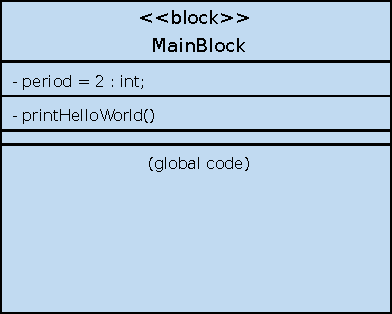
\includegraphics[scale=0.65]{figures/bdhelloworld.pdf}
\hspace{1cm}
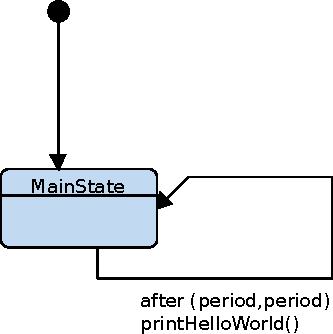
\includegraphics[scale=0.65]{figures/smdhelloworld.pdf}
\caption{Hello world model} \label{fig:printhelloworld}
\end{figure*}

You may then check the syntax of the diagram, and select the "interactive simulation icon". From the window that opens, make a step-by-step simulation, and observe the behaviour of the system. This behaviour is simulated, that is, there is no executable code that is generated to simulate the model.

\begin{figure*}[htbp]
\centering
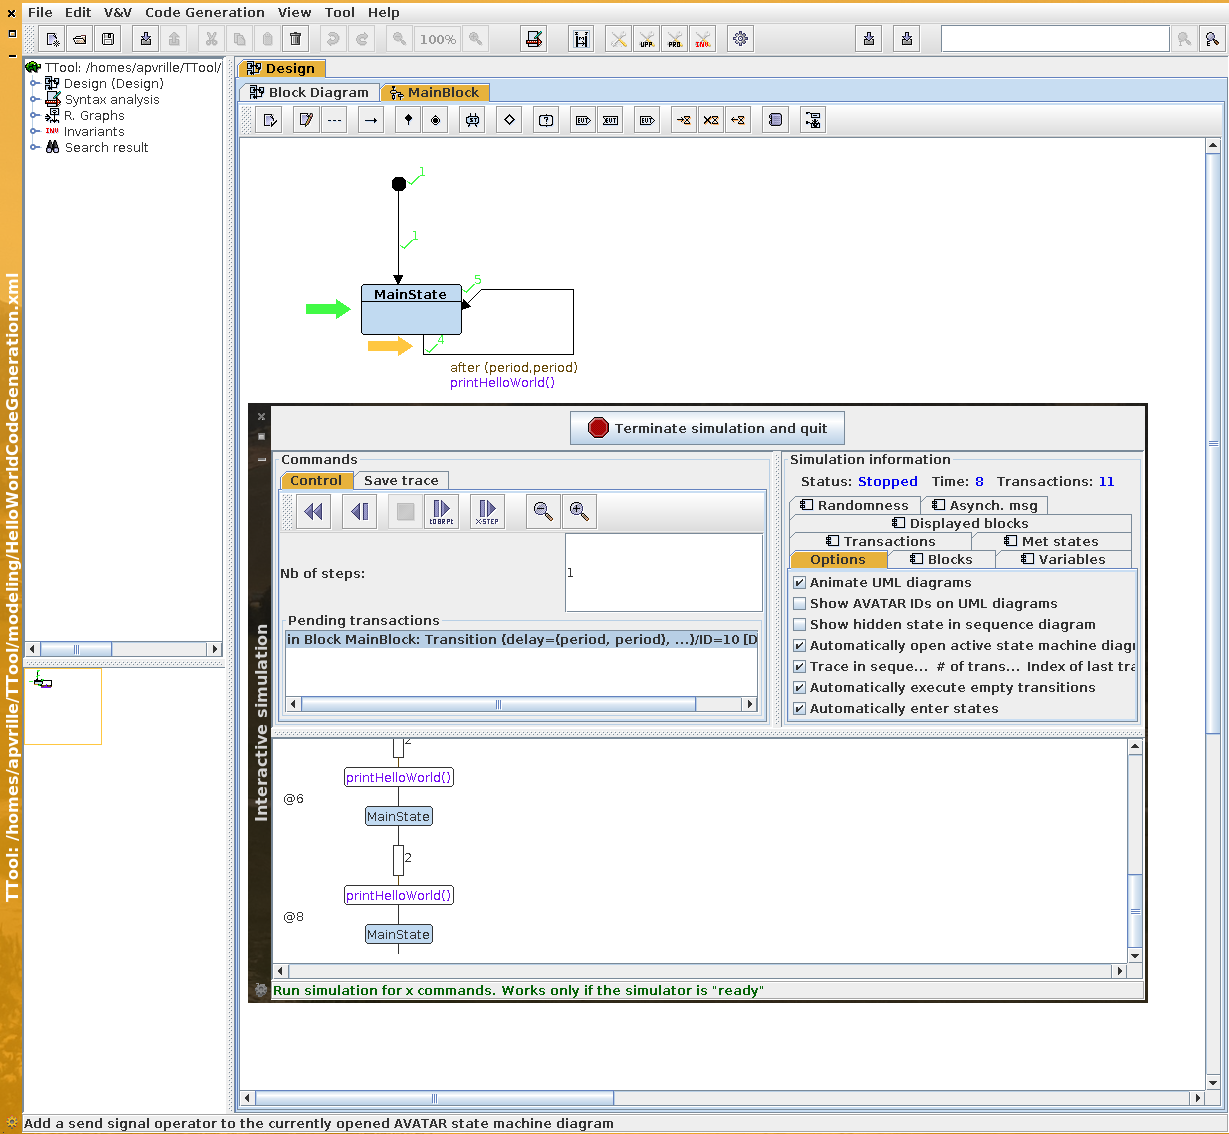
\includegraphics[width=1\textwidth]{figures/simulationhelloworld}
\caption{Functional simulation of the Hello world model} \label{fig:simuhelloworld}
\end{figure*}

\subsection{Generating executable code}
To generate executable code, click on the "check syntax" icon, and then click on the "code generation" icon representing a gear. The following window should open (see Figure \ref{fig:codegenhelloworld}).

\begin{figure*}[htbp]
\centering
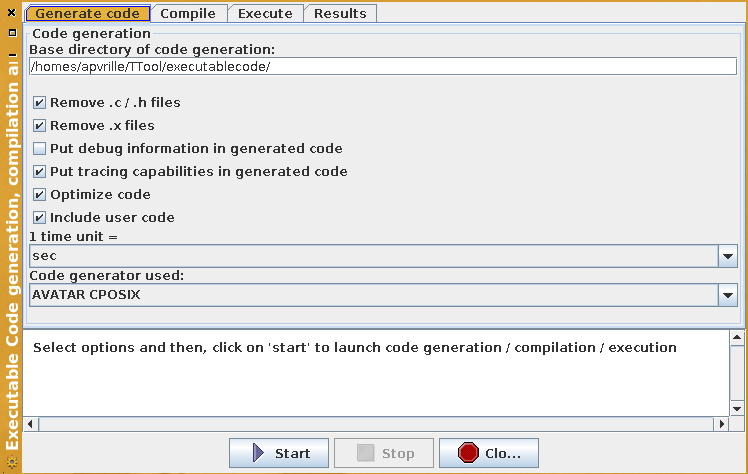
\includegraphics[width=0.9\textwidth]{figures/codegenhelloworld}
\caption{Generating C/POSIX code for the Hello world model} \label{fig:codegenhelloworld}
\end{figure*}

\begin{itemize}
\item You can add debugging information to the generating code ("Put debug information \ldots") if you wish the generated code to print information in the default output when executing. Typical debugging information is: state entering/exiting and send / receive of signals.
\item Tracing capabilities enable to draw a sequence diagram representing the execution of the code.
\item User defined code can be included (or not). \textbf{Uncheck this option first}.
\item The time unit manipulated by TTool can be set to seconds, milliseconds or microseconds. For example, if "sec" is selected, it means that  "after(2)" will be transformed as a waiting of two seconds. Default is "sec", keep it like this for the incoming tutorial.
\end{itemize}

\subsection{Compiling the generated code}
Once the code has been generated, the dialog window should automatically switch to the "Compile" tab (see Figure \ref{fig:compilehelloworld}). There, you should notice two alternative possibilities:
\begin{itemize}
\item Compile the code for your localhost (\textbf{You should select this option}).
\item Compile the code for the SoCLib platform. This option is not addressed in this document.
\end{itemize}
If the compilation fails, it is probably due to a bad installation of a C compiler. You could also edit the Makefile you have selected (see section \ref{sec:conf}) to adapt it to your localhost particularities.  Note that the compilation process also compiles the Avatar runtime C sources\footnote{These sources are located in TTool/executablecode/src}, and links all resulting object files together.

\begin{figure}[htbp]
\centering
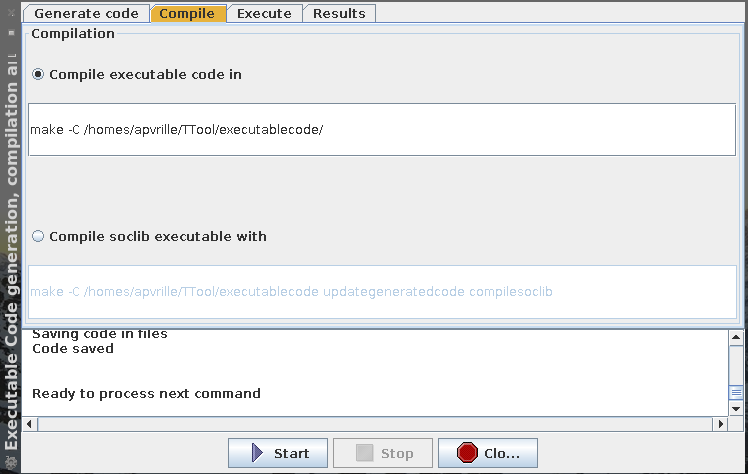
\includegraphics[width=0.9\textwidth]{figures/compilehelloworld}
\caption{Compiling the Hello world model generated C code} \label{fig:compilehelloworld}
\end{figure}

You may obvisouly try to compile the code from a terminal. e.g.:
\begin{lstlisting}
$ cd TTool/executablecode
$ make
echo Making directories
Making directories
mkdir -p ./lib
mkdir -p ./lib/generated_src/
mkdir -p ./lib/src/ 
/usr/bin/gcc -O1 -pthread -Wall  -I. -I. -Isrc/  -Igenerated_src/ -o lib/generated_src/main.o -c generated_src/main.c
/usr/bin/gcc -O1 -pthread -Wall  -I. -I. -Isrc/  -Igenerated_src/ -o lib/generated_src/MainBlock.o -c generated_src/MainBlock.c
/usr/bin/gcc -O1 -pthread -Wall  -I. -I. -Isrc/  -Igenerated_src/ -o lib/src/request.o -c src/request.c
/usr/bin/gcc -O1 -pthread -Wall  -I. -I. -Isrc/  -Igenerated_src/ -o lib/src/message.o -c src/message.c
/usr/bin/gcc -O1 -pthread -Wall  -I. -I. -Isrc/  -Igenerated_src/ -o lib/src/myerrors.o -c src/myerrors.c
/usr/bin/gcc -O1 -pthread -Wall  -I. -I. -Isrc/  -Igenerated_src/ -o lib/src/debug.o -c src/debug.c
/usr/bin/gcc -O1 -pthread -Wall  -I. -I. -Isrc/  -Igenerated_src/ -o lib/src/syncchannel.o -c src/syncchannel.c
/usr/bin/gcc -O1 -pthread -Wall  -I. -I. -Isrc/  -Igenerated_src/ -o lib/src/asyncchannel.o -c src/asyncchannel.c
/usr/bin/gcc -O1 -pthread -Wall  -I. -I. -Isrc/  -Igenerated_src/ -o lib/src/request_manager.o -c src/request_manager.c
/usr/bin/gcc -O1 -pthread -Wall  -I. -I. -Isrc/  -Igenerated_src/ -o lib/src/random.o -c src/random.c
/usr/bin/gcc -O1 -pthread -Wall  -I. -I. -Isrc/  -Igenerated_src/ -o lib/src/mytimelib.o -c src/mytimelib.c
/usr/bin/gcc -O1 -pthread -Wall  -I. -I. -Isrc/  -Igenerated_src/ -o lib/src/tracemanager.o -c src/tracemanager.c
/usr/bin/gcc -O1 -pthread -ldl -lrt -Wall  -I. -I. -Isrc/  -Igenerated_src/ -L. -L..  -o run.x lib/generated_src/main.o lib/generated_src/MainBlock.o lib/src/request.o lib/src/message.o lib/src/myerrors.o lib/src/debug.o lib/src/syncchannel.o lib/src/asyncchannel.o lib/src/request_manager.o lib/src/random.o lib/src/mytimelib.o lib/src/tracemanager.o -lm  2>&1 | c++filt
\end{lstlisting}

\subsection{Executing the generated code}
Once the generated code has been successfully compiled and linked, the execution tab is selected (see Figure \ref{fig:executehelloworld}). There are three possible options to execute the compiled program:
\begin{figure}[htbp]
\centering
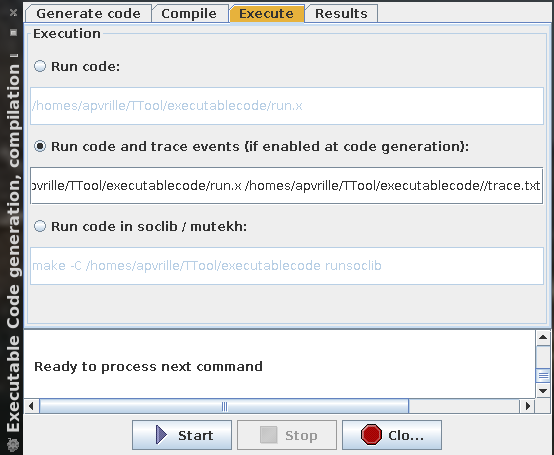
\includegraphics[width=0.9\textwidth]{figures/executehelloworld}
\caption{Executing the Hello world program} \label{fig:executehelloworld}
\end{figure}

\begin{itemize}
\item Running the program ("Run code")
\item Running the program and activating the backtracing
\item Running the program in the SoCLib environment (no covered in this document).
\end{itemize}
Select the second option. An execution trace should be displayed in the console of the dialog window.

\subsection{Backtracing}
After you have started the program, switch to the "Results" tab. You should see a window similar to the one display in Figure \ref{fig:resultshelloworld}. There are two options:
\begin{figure}[htbp]
\centering
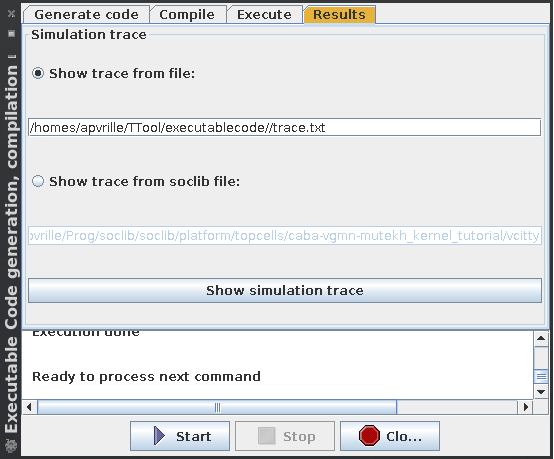
\includegraphics[width=0.9\textwidth]{figures/resultshelloworld}
\caption{Backtracing dialog window} \label{fig:resultshelloworld}
\end{figure}
\begin{itemize}
\item Displaying the execution trace of the localhost program
\item Displaying the execution trace of the SoCLib program (option is not covered in this manual)
\end{itemize}
Select the first option, and click on the "show simulation trace" button. A new window should open, displaying the execution of the model under the form of a UML Sequence Diagram (see Figure \ref{fig:backtracinghelloworld})

\begin{figure}[htbp]
\centering
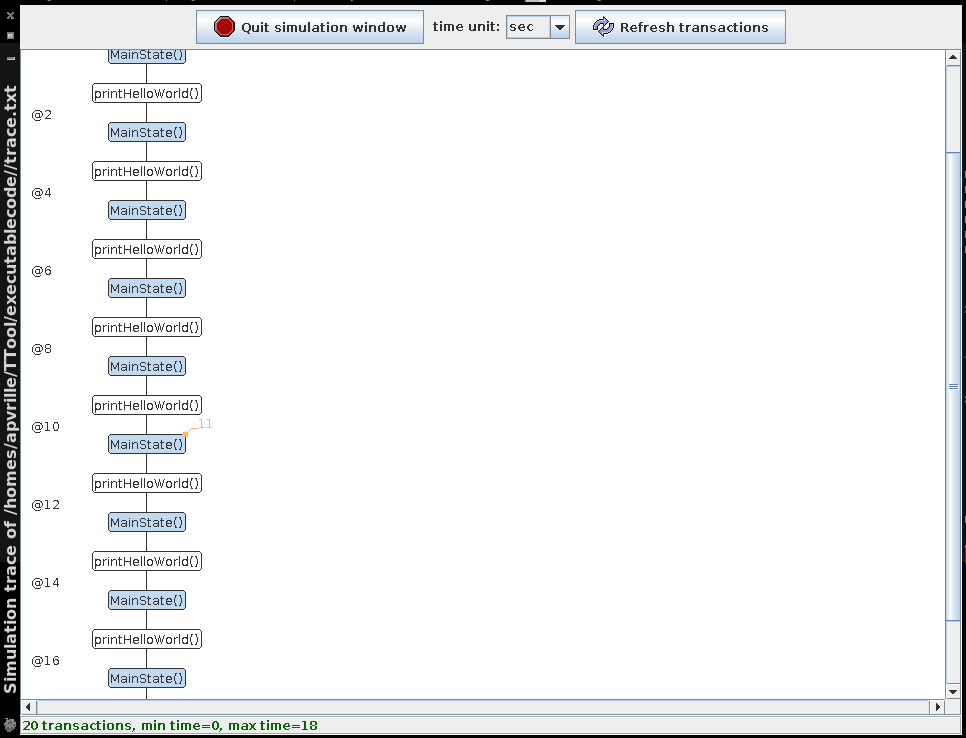
\includegraphics[width=0.9\textwidth]{figures/backtracinghelloworld}
\caption{Executing the Hello world program} \label{fig:backtracinghelloworld}
\end{figure}

\newpage
\section{Enhancing model with user code}\label{sec:custom}

\subsection{Principle}
A user of TTool can provide its own C code within an AVATAR design diagram. When a model is enhanced with custom C code, the custom C code may prevent the compilation process to succeed: if the compilation fails, you need to reconsider the code you have inserted according to the errors provided by the compiler.\\
Basically, there are two types of custom code as show in the "prototyping" window (see Figure \ref{fig:customhelloworld}). To open this window, simply double-click in the attributes/methods/signal/code part of a given block.
\begin{itemize}
\item \textbf{The global code of the model}
\item \textbf{The local code of a given block}. This code is itself split into two sub parts:
\begin{itemize}
\item The global code of the block.
\item The code implementing methods of the block.
\end{itemize}
\end{itemize}

\begin{figure}[htbp]
\centering
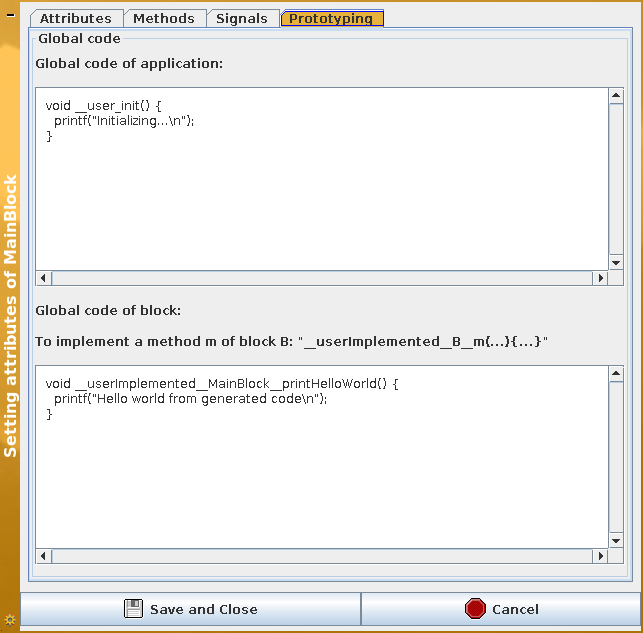
\includegraphics[width=0.9\textwidth]{figures/customhelloworld}
\caption{Executing the Hello world program} \label{fig:customhelloworld}
\end{figure}

\subsection{Global code}
The global code typically contains the declaration of global variables. Also, one specific method can be used to execute code when the application starts. The function prototype is: 
\begin{verbatim}
void __user_init()
\end{verbatim}
For instance, the global code of the HelloWorld example is as follows:
\begin{lstlisting}
void __user_init() {
  printf("Initialializing\n");
}
\end{lstlisting}

\subsection{Block code}
The block code typically contains variables that are not declared as block attributes. Block attributes can indeed be directly used in the custom code. The block code can also provide an implementation for the block methods. For a method called "method" of the block "block", the function must be declared as "\_userImplemented\_block\_method" and \textbf{you must ensure to check the "Implementation provided by the user" option} in the method definition window (see Figure \ref{fig:methodhelloworld}). For instance, the following code correesponds to the block code of "MainBlock". It implements the method \textit{printHelloWorld()} referenced in the model (see Figure \ref{fig:printhelloworld}).
\begin{lstlisting}
void _userImplemented_MainBlock__printHelloWorld() {
  printf("Hello world from generated code\n");
}
\end{lstlisting}

\begin{figure}[htbp]
\centering
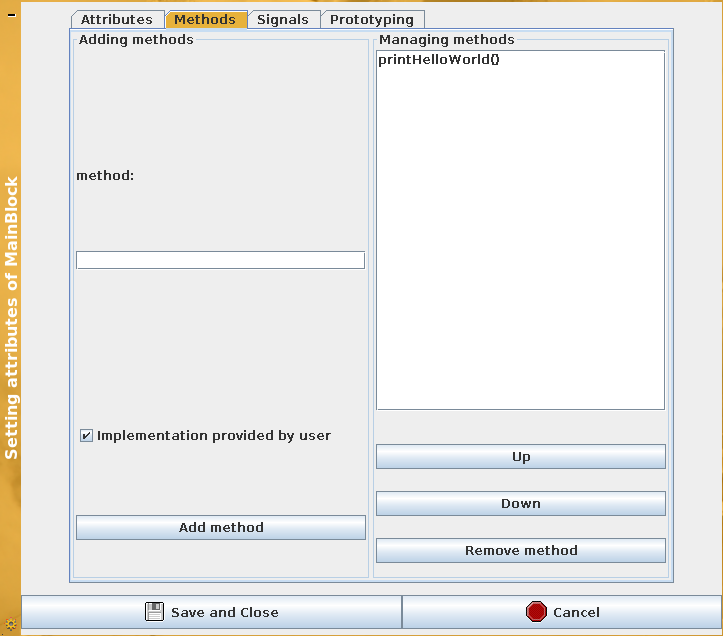
\includegraphics[width=0.9\textwidth]{figures/methodhelloworld}
\caption{Selecting a method for which the user provides an implementation}\label{fig:methodhelloworld}
\end{figure}

\subsection{Code generation and execution with custom code}

Be sure to \textbf{check the "Include user code" option} on the code generation tab of the code generation window. You may also uncheck the "Put tracing capabilities in generated code" since we won't use this in this example. Then, follow the usual stages: compile, and then execute the program. You should now see the effect of the printf command in the console. It should like this:
\begin{lstlisting}
Initializing...
Hello world from generated code
Hello world from generated code
Hello world from generated code
\end{lstlisting}

\newpage
\section{Advanced model enhancement with user code}\label{sec:advanced}
To follow this section, you have to use another TTool model called "MicroWaveOven\_SafetySecurity\_fullMethodo.xml", available on the network repository of TTool (File, Open from TTool repository).\\
This section explains how a code generated from TTool can be linked with an external software, e.g. to animate a graphical user interface. The provided example relies on datagrams and sockets to echange information between the Microwave Software (fully generated from TTool) and its graphical user interface (programmed "by hand"). We will now call these two software MS and GUI, respectively

\subsection{GUI}
The TTool distribution includes an external software which represents a graphical user interface of a microwave system. The source code (in Java) of this software is located in "TTool/executablecode/example":
\begin{lstlisting}
$cd TTool/executablecode/example
$ ls
DatagramServer.java  Feeder.java  MainMicrowave.java  MicrowavePanel.java  README
\end{lstlisting}
This directory contains the java sources as well as a README file. First compile the java source code, and then execute the GUI, as follows:
\begin{lstlisting}
$javac *.java
$java MainMicrowave
\end{lstlisting}
A window similar to the one of Figure \ref{fig:gui1} should open. This window is not yet animated. To do so, we need to build the MS.

\begin{figure}[htbp]
\centering
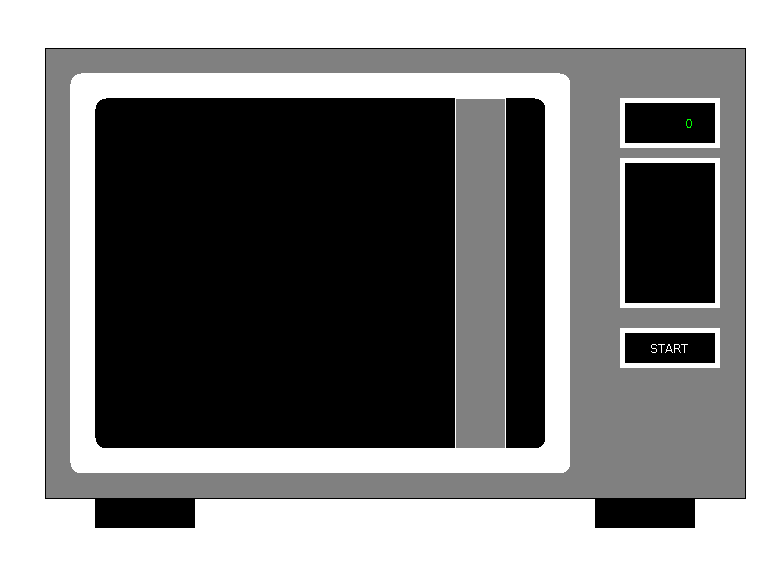
\includegraphics[width=0.9\textwidth]{figures/gui1}
\caption{Window of the Graphical User Interface} \label{fig:gui1}
\end{figure}

\subsection{Microwave Software (MS)}
Open the model in TTool, then double-click on a block method, and finally select the "Prototyping" tab. You can now review the global and local code.
\subsubsection{Global code}
The goal of the global code is to setup the communication infrastructure to the GUI. To do so, the global code is as follows.
\begin{itemize}
\item It declares headers.
\begin{lstlisting}
#include <sys/types.h>
#include <sys/socket.h>
#include <netinet/in.h>
#include <netdb.h>
#include <stdio.h>
#include <strings.h>
#include <errno.h>
\end{lstlisting}

\item It defines the global constants and variables, including the hostname to use, and the port.
\begin{lstlisting}
const char* hostname="localhost";
const char* portname="8374";
int fd;
struct addrinfo* res;
\end{lstlisting}

\item It defines a function to send a datagram.
\begin{lstlisting}
void sendDatagram(char * data, int size) {
  if (sendto(fd,data,size, 0, res->ai_addr,res->ai_addrlen)==-1) {
        printf("Error when sending datagram");
        exit(-1);
    }
}
\end{lstlisting}
\item It defines the user initialization function. This function puts in an "addinfo struct" information for sending the datagram. Then, it gets the target IP address. Following this, it creates a reference to the right socket. Finally, it tries to send a test packet ("salut"). Whenever a failure is encountered, the application exits. When the C code is generated from the model, all the global code is integrated into a file called "main.c".
\begin{lstlisting}
void __user_init() { 
  const char* content = "salut";
  struct addrinfo hints;

  memset(&hints,0,sizeof(hints));
  hints.ai_family=AF_UNSPEC;
  hints.ai_socktype=SOCK_DGRAM;
  hints.ai_protocol=0;
  hints.ai_flags=AI_ADDRCONFIG;
 
  int err=getaddrinfo(hostname,portname,&hints,&res);
  if (err!=0) {
    printf("failed to resolve remote socket address (err=%d)",err);
    exit(-1);
  }
  fd=socket(res->ai_family,res->ai_socktype,res->ai_protocol);
  if (fd==-1) {
    printf("%s",strerror(errno));
    exit(-1);
  }
  if (sendto(fd,content,sizeof(content),0,
      res->ai_addr,res->ai_addrlen)==-1) {
    printf("%s",strerror(errno));
    exit(-1);
  }

}
\end{lstlisting}
\end{itemize}
Note: the network code of the GUI application is located in \textit{DatagramServer.java}.

\subsubsection{Local code}
The local code associates the call to a method of a block to the sending (or receiving) of a datagram packet. Let's take the example of the "Door" block. The GUI should be informed about door opening or closing operations. In the model, each time the door is closed, the \textit{openM()} method is closed. Also, each time the door is closed, the \textit{closeM() }method is called (see Figure \ref{fig:door}).

\begin{figure}[htbp]
\centering
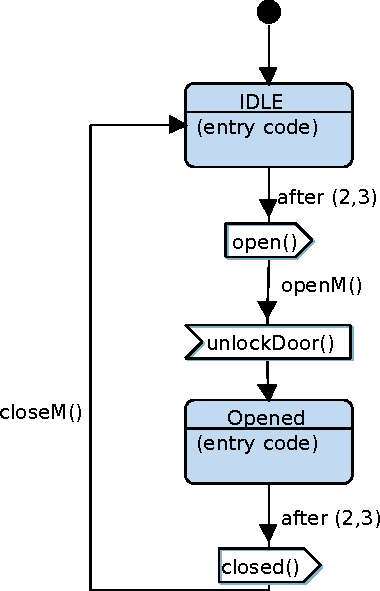
\includegraphics[width=0.4\textwidth]{figures/door}
\caption{State Machine Diagram of the Door block} \label{fig:door}
\end{figure}

In the local code, we first need to state that a \textit{sendDatagram()} function is externally defined.
 \begin{lstlisting}
extern void sendDatagram(char *data, int size);
\end{lstlisting}
Then, we need to define the user defined C code for both \textit{openM()} and \textit{closeM()}.  We also define constant strings in order to uniquely identifiydatagram packets sent to the GUI. In the code, "10" corresponds to the length of the datagram. 

\begin{lstlisting}
const char* openD = "Open Door";
const char* closeD = "Close Door";

void _userImplemented_Door__openM() {
  sendDatagram(openD, 10);
}

void _userImplemented_Door__closeM() {
   sendDatagram(closeD, 10);
}
\end{lstlisting}

The corresponding packets are also defined in the GUI application e.g. see \textit{MainMicrowave.java}. 

\subsection{GUI animation}
Generate the C code from TTool (be sure to check the "Include user code" option). Start the GUI from a terminal, and then, start the MS application from TTool (you can also start MS from a terminal). You should see the animations of the GUI while the generated application executes. For example, Figure \ref{fig:animopen} shows the microwave when the door opened, and Figure \ref{fig:animcooking} shows the microwave in heating mode.

\begin{figure}[htbp]
\centering
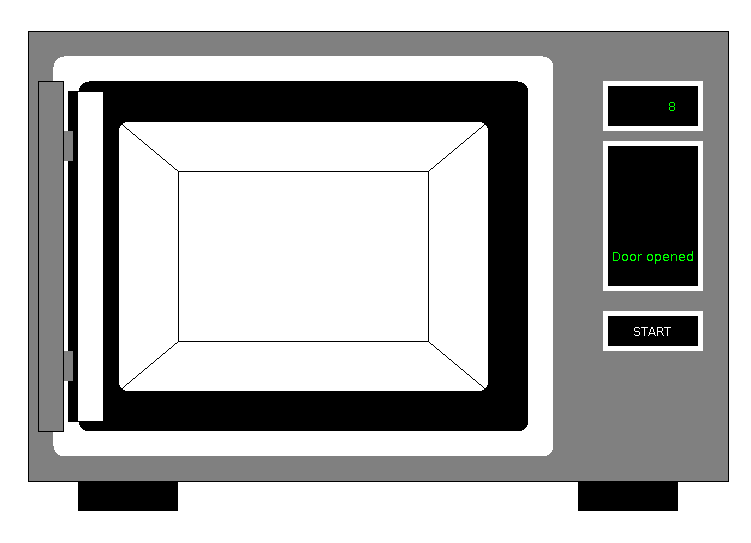
\includegraphics[width=0.5\textwidth]{figures/animopen}
\caption{GUI when the door is opened} \label{fig:animopen}
\end{figure}

\begin{figure}[htbp]
\centering
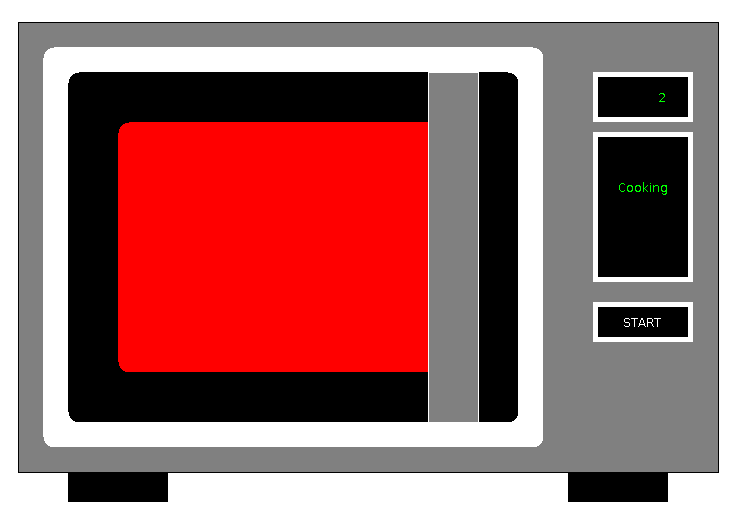
\includegraphics[width=0.5\textwidth]{figures/animcooking}
\caption{GUI when the microwave is cooking} \label{fig:animcooking}
\end{figure}


\newpage
\section{Customizing the code generator}\label{sec:customgenerator}
We are currently working on a plug-in facility in order to be able to customize the AVATAR-to-C code generator. Send us an email to be informed about updates, or stay connected to \url{https://twitter.com/TTool_UML_SysML}
\end{document}
